\chapter{System Architectural Design}
\section{System Components}
This chapter seeks to identify the system components. It provides a block definition diagram (bdd) of the system, where the system components are determined along with the static relationship between them. The block definition diagram is shown in figure \ref{fig:block_diagram}:
\begin{figure}[H]
\centering
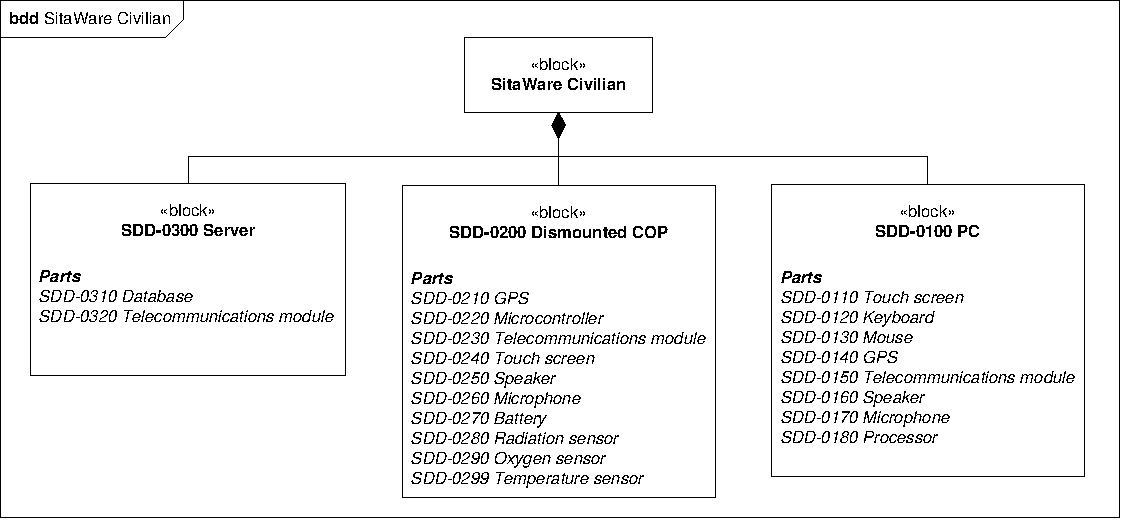
\includegraphics[width=0.95\textwidth]
{billeder/bdd_overordnet.pdf}
\caption{Block diagram of the system.}
\label{fig:block_diagram}
\end{figure}
The diagram consists of system-blocks along with parts associated to each block. The system-blocks are depicted as two-compartment blocks with the name of the block in the first compartment, and sub parts in the second compartment. In the next section, a short description of each system-block is given.
\subsection{Component description}
\begin{enumerate}
\item[•] \textbf{PC:} This block constitutes the machine in the head quarter (HQ) on which the COP-software will be executed. It also has a GPS module, so that the location of the HQ is always known. The PC has a telecommunication module, in order to be able to communicate with the rest of the system.
\item[•] \textbf{Server:} The server will facilitate communication between the other blocks. In addition, it will store user information along with logs locally in an internal database.
\item[•] \textbf{Dismounted COP:} This block constitutes the machine on which the condensed COP-software will be executed. The dismounted COP will be used by the dismounted users in the field. It has a GPS module, so that the location of the dismounted users is always known. Furthermore it has a telecommunication module so that it will be able to communicate with the rest of the system. 
\end{enumerate}
\section{Concept of Execution}
\section{Interface Design}

This section seeks to describe the interface characteristics of the system components. It provides an internal block diagram (bdd) of the system, where the interfaces of the system components are identified, as long as the external interfaces of the system. The internal block diagram of the overall system is shown in figure \ref{fig:internal_block_diagram}:
\begin{figure}[H]
\centering
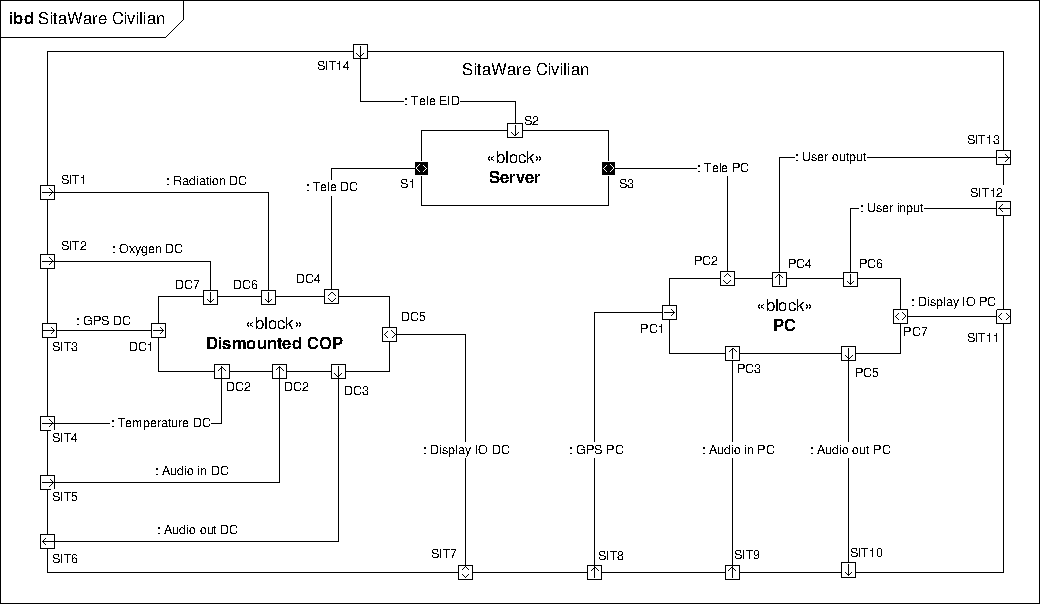
\includegraphics[width=0.95\textwidth]
{billeder/ibd_overordnet.pdf}
\caption{Internal block diagram of the system.}
\label{fig:internal_block_diagram}
\end{figure}


\begin{table}[H]  
\centering

\begin{tabular}{|l|p{8cm}|l|l|} 
\hline
	\textbf{Name}		& \textbf{Description}						  & \textbf{Port 1} & \textbf{Port 2} \\\hline
  Radiation DC				&  Radiation level to the dismounted COP 	 					   & SIT1 & DC6 \\\hline
  Oxygen DC					&  Oxygen level signal to the dismounted COP				   & SIT2 & DC7 \\\hline
  GPS DC					&  GPS signal for the dismounted COP 	 					   & SIT3 & DC1 \\\hline   
  Temperature DC			&  Temperature signal to the dismounted COP 	 					   & SIT4 & DC2 \\\hline     
  Audio in DC				&  Microphone for communication purposes 	 				   & SIT5 &\textbf{ DC8  FIX PÅ DIAGRAM!!!!!}\\\hline     
  Audio out DC				&  Speaker for communication purposes 	 					   & SIT6 & DC3 \\\hline     
  Display IO DC				&  Display input/output for dismounted COP 	 					   & SIT7 & DC5 \\\hline     
  
  GPS PC					&  GPS signal for the PC			 	 					   & SIT8 & PC1 \\\hline     
  Audio in PC				&  Microphone for communication purposes 	 					   & SIT9 & PC3 \\\hline     
  Audio out PC				&  Speaker for communication purposes 	 					   & SIT10 & PC5 \\\hline     
  Display IO PC				&  Display input/output for PC 	 					   & SIT11 & PC7 \\\hline     
  Keyboard PC				&  Keyboard input to the PC 	 					   & SIT12 & PC6 \\\hline     
  Mouse in PC				&  Mouse input to the PC 	 					   & SIT13 & PC4 \\\hline    
  Tele EID S				&  \textbf{MANGLER !!!} 					   & SIT14 & S2 \\\hline
       
  Tele DC					&  Telecommunication between the dismounted COP and the server & DC4 & S1 \\\hline   
  Tele 						&  Telecommunication between the PC and the server 					   & PC2 & S2 \\\hline   
   
\end{tabular}
\caption {General ibd} 
%\label{} 
\end{table} 







\subsection{PC}
In this section the internal interfaces of the PC to be used in this system are specified in greater detail. All the sub parts of the PC are connected to the processor which manages all logic operations and functions, while the telecommunication module enables the PC to communicate with the remaining system components. It is not within the scope of this project to develop the PC itself, however the COP is to be executed on the PC. Therefore the interfaces of the PC are identified, to ensure that the PC - and thereby the COP - can communicate with the rest of the system. The internal block diagram of the PC is shown in figure \ref{fig:internal_diagram_PC}:
\begin{figure}[H]
\centering
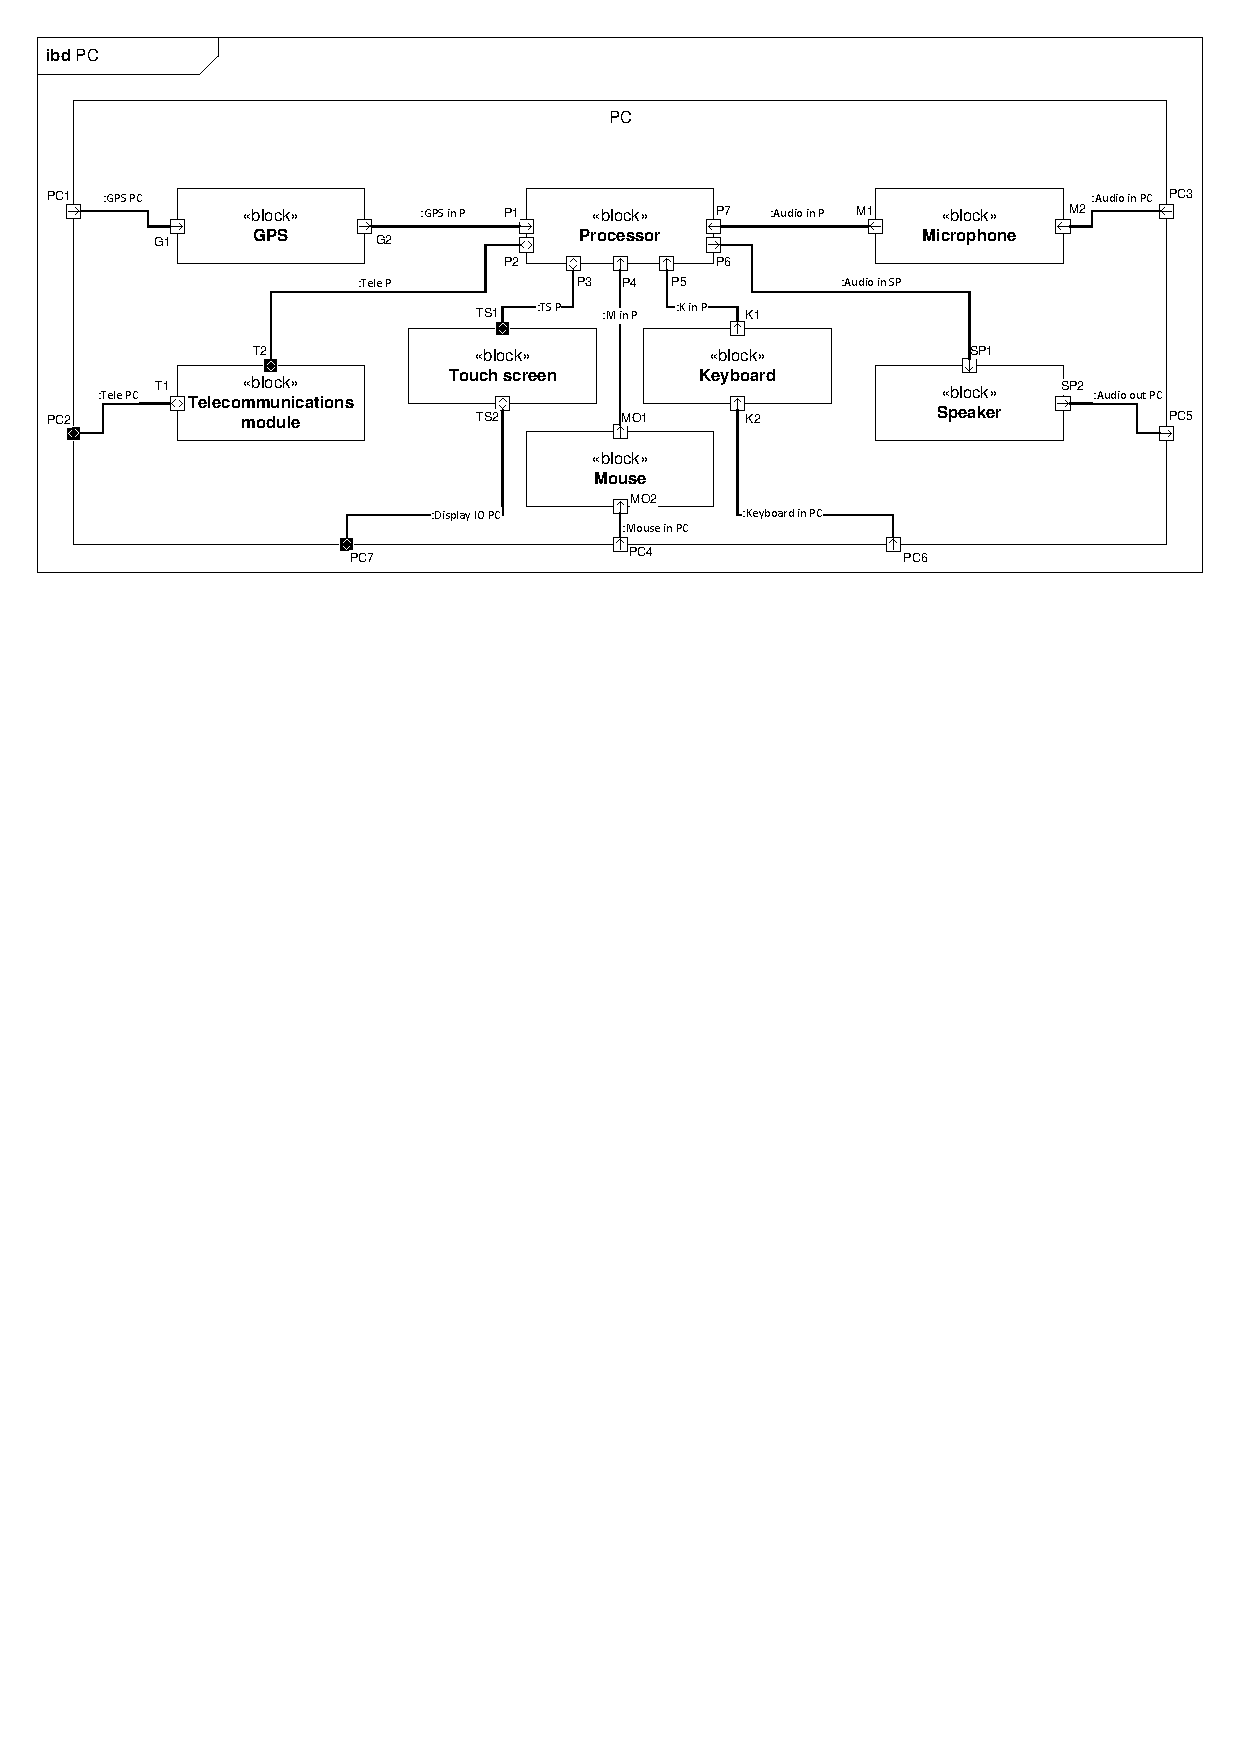
\includegraphics[width=0.95\textwidth]
{billeder/ibd_PC.pdf}
\caption{Internal block diagram of the PC.}
\label{fig:internal_diagram_PC}
\end{figure}


\begin{table}[H]  
\centering

\begin{tabular}{|l|p{8cm}|l|l|} 
\hline
	\textbf{Name}		& \textbf{Description} & \textbf{Port 1} & \textbf{Port 2} \\\hline
GPS DC	    & Dismounted COP receiving GPS signal												 & G1 &  PC1 \\\hline
Tele PC     & Telecommunication between the PC and the server							   		 & T1 &  PC2 \\\hline		
Audio in PC & Microphone for communication purposes  											 & M2 &  PC3 \\\hline				  
Mouse in PC	    & Input from the mouse										 					 & MO2 &  PC4\\\hline				  
Audio out PC	        & Speaker for communication purposes 			  						 & SP2 & PC5 \\\hline			
Keyboard in PC	& Input from the keyboard   				 				 					 & K2 &  PC6 \\\hline				  
Display IO PC	& Input and output from user to the touch screen								 & TS2 &  PC7 \\\hline				  
	
GPS in P	& Signal from the GPS to the processor								                 & P1 & G2 \\\hline				  			
Tele P		& Communication between the telecommunications module and the processor              & P2 & T2 \\\hline				  			
TS P		& Communication between the touch screen module and the processor          			 & P3 & TS1 \\\hline			  			
M in P		& Signal from the mouse to the processor          								     & P4 & MO1 \\\hline				  	
K in P		& Signal from the keyboard to the processor          								 & P5 & K1 \\\hline				  			
Audio in SP	& Signal from the processor to the speaker					             			 & P6 & SP1 \\\hline				  		Audio in P	& Signal from the microphone to the processor					           		     & P7 & M1 \\\hline				  			
												   
\end{tabular}
\caption {Dismounted COP ibd} 
%\label{} 
\end{table} 





When looking into the PC the different modules are displayed on the ibd. The connections between the modules describes the data flow. In the PC a processor is connecting all the units together, while the telecommunication module is connecting the PC to the other devices. The i/o from the microphone, speakers, touch screen, mouse and keyboard reaches to the physical world to connect with the user.
\section{Concept of execution}

\begin{figure}[H]
\centering
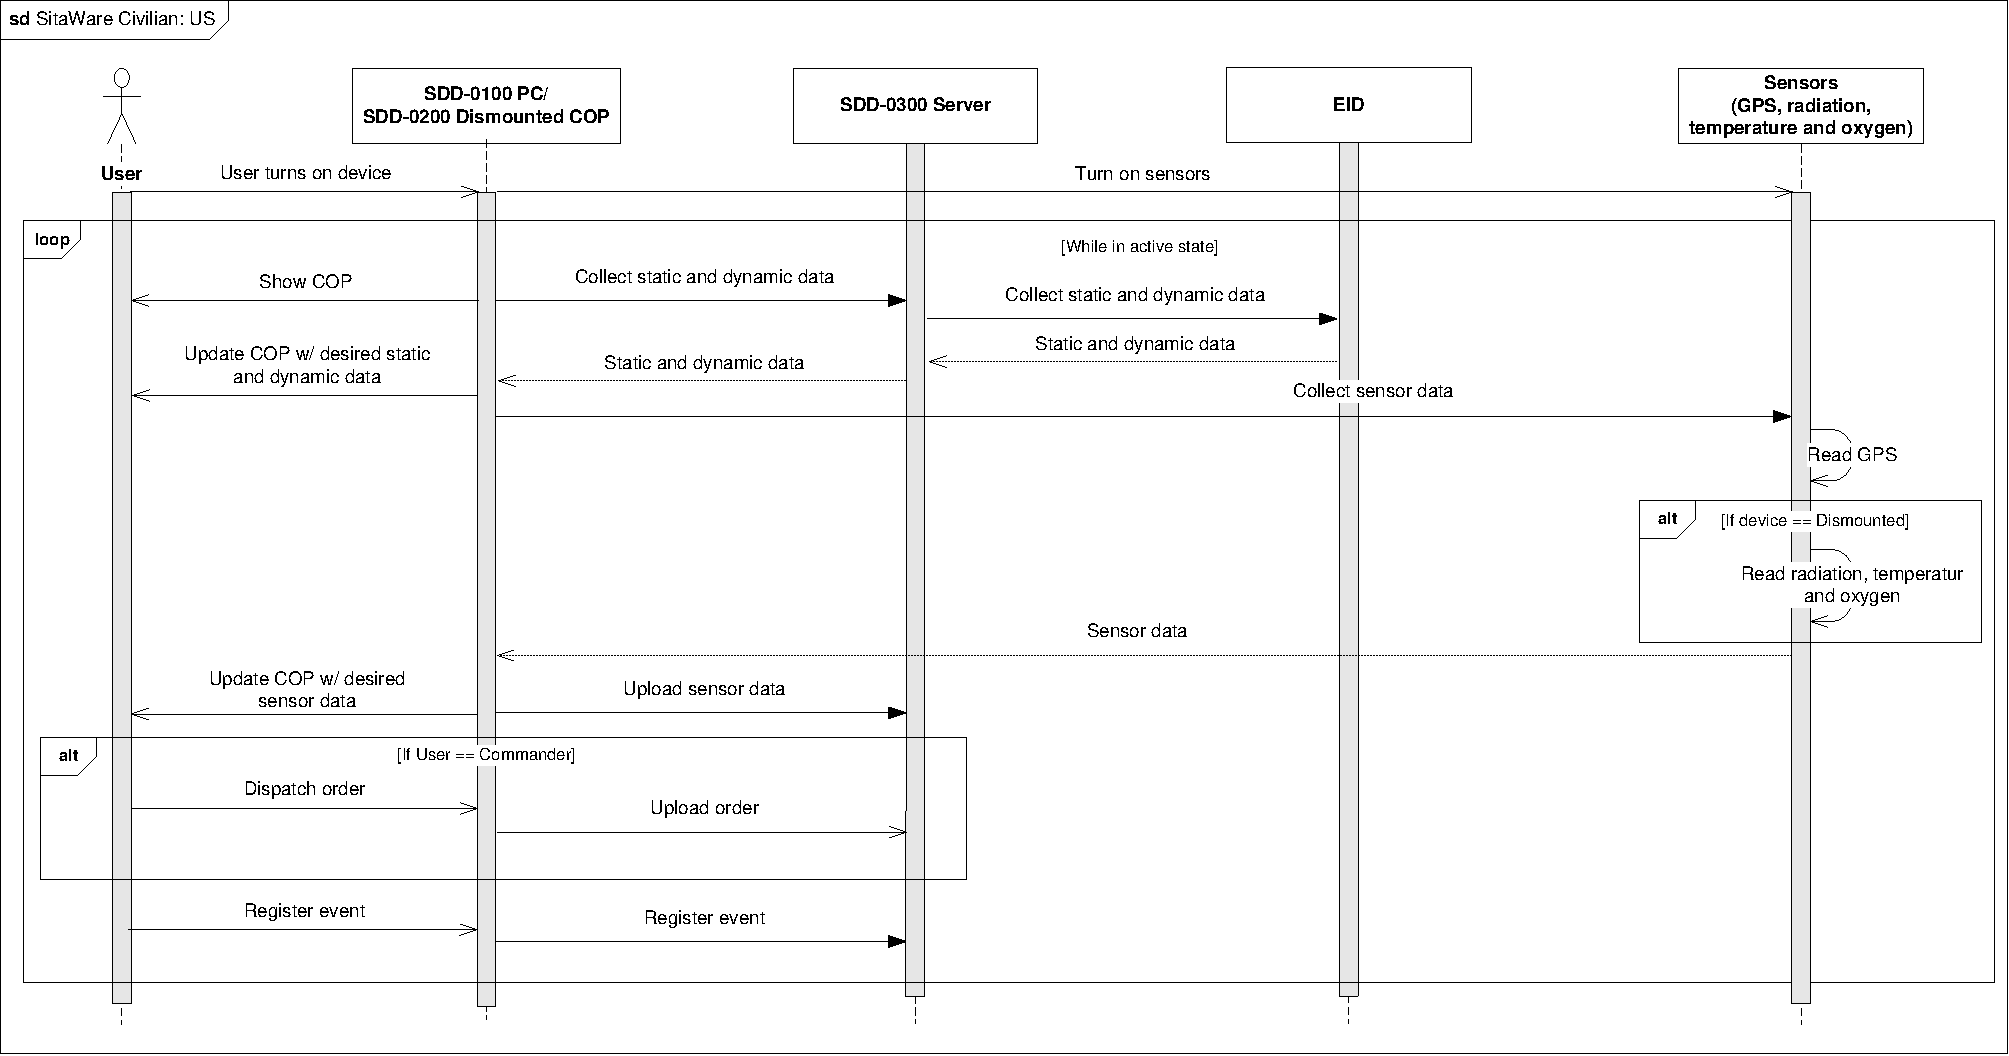
\includegraphics[width=0.95\textwidth]
{billeder/sekvens1.pdf}
\caption{Overall sequence diagram for SitaWare Civilian.}
\label{fig:sekvens1}
\end{figure}

